\section{WebStat Unit}
\label{sec:webclient}

\emph{WebStat} unit is output type unit that connects to BGPmon. \emph{WebStat} unit receive stream of XML messages from BGPmon. In particular, \emph{WebStat} unit filters BGPmon's stream of XML messages to process only those messages that corresponds to XML \emph{Status} messages. XML \emph{Status}  messages include information  from three types of input to BGPmon: \emph{Peer}, \emph{MRT} and \emph{Chain} units. \emph{Peer} and \emph{MRT} units provide a detailed summary about peering sessions, memory usage, number of received BGP messages and others. \emph{Chain} unit provide information about connected chain instances.   \emph{WebStat} unit use data from all 3 inputs to create a HTML report and user of framework may use it to monitor the state of  BGPmon. 

In order to use \emph{WebStat}, user of framework need to be familiar with design of \emph{WebStat} unit.   \emph{WebStat} unit is a set of two applications: \emph{StatClient} and \emph{WebGen}. \emph{StatClient} is application that connects to BGPmon instance and retrieve XML data. Also, it filters \emph{Status} messages from entire set of XML messages. \emph{Status} messages contain information about \emph{Peer}, \emph{MRT} and \emph{Chain} units. \emph{StatClient}  periodically saves filtered data to the filesystem. \emph{WebGen} is an application that use data from filesystem to generate HTML page that includes statistical data and figures that shows changes over the time. In order to have the most current information from \emph{Peer}, \emph{MRT} and \emph{Chain} input sources \emph{WebGen} runs in crontab scheduler and periodically updates HTML page. 

\emph{WebStat} unit is designed to achieve following goals:

\begin{itemize}
\item{BGPmon provide XML messages in output: its important to verify that BGPmon is able to send  stream of XML messages to \emph{WebStat} unit .}
\item{Generate Statistics: HTML report shows summary of \emph{Peer}, \emph{MRT} and \emph{Chain} units.}
\end{itemize}

\subsection{IPv4 WebStat Unit}

\begin{figure}
\centering
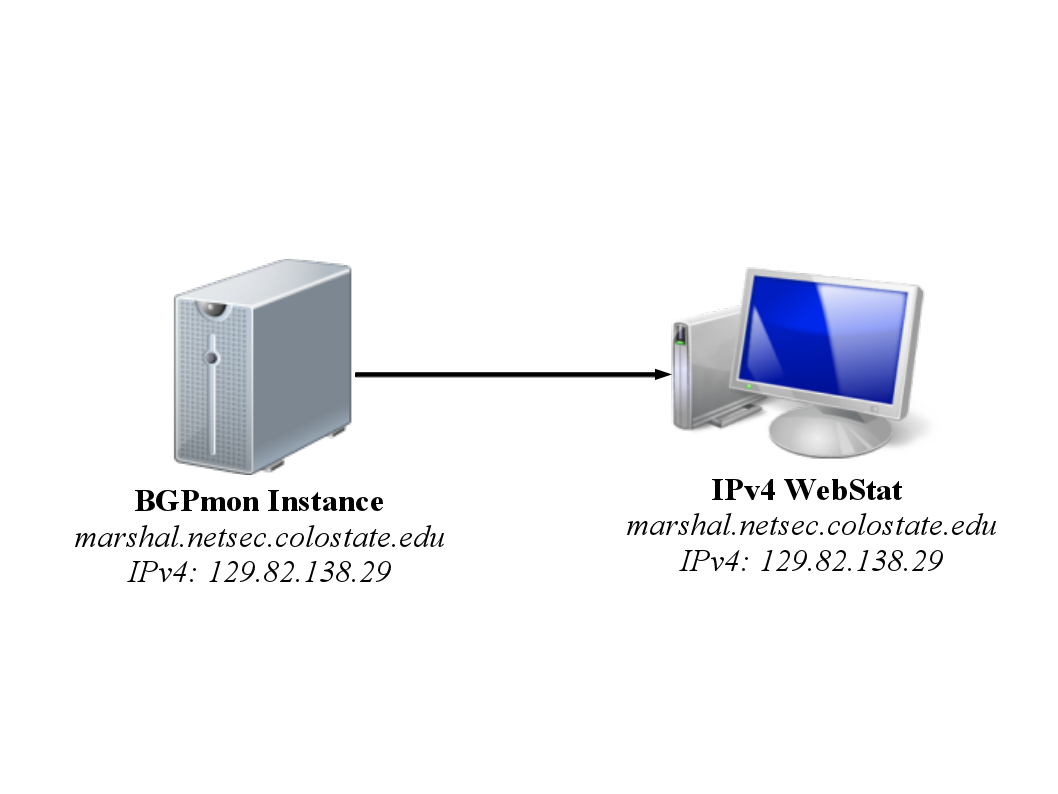
\includegraphics[scale=0.30]{figs/ipv4-webstat.png}
\caption{An overview of IPv4 WebStat Unit.}
\label{webstat}
\end{figure}

Figure \ref{webstat} shows unit design: it has \emph{IPv4 WebStat} unit and BGPmon test instance. Both \emph{IPv4 WebStat} unit and BGPmon test instance are installed on same host \emph{marshal.netsec.colostate.edu} with \emph{129.82.138.29} IPv4 address. 

\subsubsection{IPv4 WebStat Unit Configuration}

\emph{IPv4 WebStat} unit has two applications: \emph{IPv4 StatClient} and \emph{IPv4 WebGen}. 

\emph{IPv4 StatClient} is application that connects to BGPmon test instance and receives XML messages.    \emph{IPv4 Stat client} supports following input values:

\begin{verbatim}
$ statclient [IP] [PORT] [DIRECTORY]
\end{verbatim}

where \emph{[IP]} is IP address of BGPmon instance. \emph{[PORT]} is a port of BGPmon server. \emph{[DIRECTORY]} is directory on \emph{marshal.netsec.colostate.edu} where XML messages are stored. 

\emph{IPv4 WebGen} is application that uses data output from \emph{IPv4 StatClient} unit and generates a HTML report. To make HTML report, run \emph{WebGen} as follows:

\begin{verbatim}
$ webgen [SOURCE DIRECTORY] [DESTINATION DIRECTORY]
\end{verbatim}

where \emph{[SOURCE DIRECTORY]} is a directory with XML data from \emph{IPv4 StatClient} and \emph{[DESTINATION DIRECTORY]} is public html directory where HTML will be saved. 

 
%WebStat Client has following configuration:
%\begin{itemize} 
%  \item{Hostname: \emph{marshal.netsec.colostate.edu}.}
%  \item{IPv4 address: \emph{129.82.138.29}.}
%\end{itemize}

%BGPmon instance has following configuration:
%\begin{itemize} 
%  \item{Hostname: \emph{marshal.netsec.colostate.edu}.}
%  \item{IPv4 address: \emph{129.82.138.29}.}
%\end{itemize}

\subsubsection{BGPmon Test Unit Configuration}

To enable  XML feed on BGPmon instance, user has to be logged to \emph{marshal.netsec.colostate.edu} and ensure that BGPmon process is up and running.  To enable stream of XML messages, run   run following command in \emph{configuration mode} in  CLI:

\begin{verbatim}
marshal(config)#client-listener enable
\end{verbatim}

BGPmon test instance starts  to listen TCP connections on \emph{50001} and \emph{50002} on \emph{marshal.netsec.colostate.edu}. Port \emph{50001} provides a stream of XML update messages, port \emph{50002} sends XML table messages.



\subsubsection{Result reporting}


WebStat Client Test Unit provide a report of extracted data from XML stream. Test unit  generates HTML page that is browsable at \url{http://bgmon.netsec.colostate.edu/framework/stat.html} page. In case of successfully received XML data,  HTML report contains information about configured peer, MRT, chain sessions that are configured at BGPmon test instance.  Overall, generated result report is beneficial in debugging problems   related to any of \emph{Peer}, \emph{MRT} or \emph{Chain} units.

%related to all tests unit described in this document.   For example, if configuration for IPv4 peering was not loaded or peers could not establish BGP session, HTML report wont have any peering statistics. Moreover, if user runs \emph{Chain Module Test Unit}, results of the test unit  are easily  visible:  HTML report shows enabled chain session with corresponding IP address, update and table ports, retry value.

